% chapter4.tex (Solution)

\chapter{Proofs}
\label{ch:sol}

This chapter includes the main proofs related to the definition of the guessing game with fractional routing. Examples of the new game are provided to help explain the concept. These examples give an insight into where the new fractional guessing game can improve on the ordinary definition of the guessing game.

\section{Examples}

\begin{figure}[ht]
	\centering
	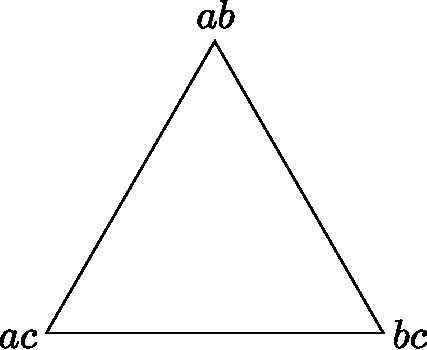
\includegraphics[width=100pt]{figures/k3.pdf}
	\caption[Resolving messages on $K_3$]{$K_3$ has $k = 3/2$ for block length $1$.}
  \label{k3}
\end{figure}

It is interesting to study the strategies that yield the highest guessing numbers for players. In Figure~\ref{k3} above, each player must resolve their own message (comprising $\log(s)$ bits) --- however, only one bit may be received from each neighbour. When comparing bits, the probability that the two are the same is $s^{-1/2}$. If three bits are fixed, then since the other three are independent, the probability that each player correctly determines their own message is $s^{-3/2}$, giving a guessing number of $k = 3/2$. In other words, this strategy succeeds with higher probability than uncoordinated random guessing, but it is not as successful as the network coding strategy.

\begin{figure}[ht]
	\centering
	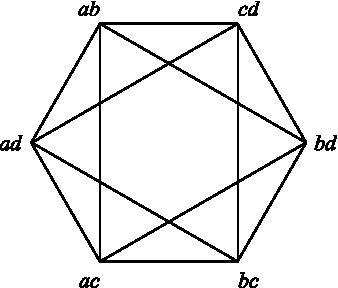
\includegraphics[width=150pt]{figures/n6.pdf}
	\caption[Optimal solutions by grouping vertices]{Grouping vertices on $Ci_6 \, (1, 2)$ yields the optimal solution.}
	\label{n6}
\end{figure}

The circulant graph $Ci_6 \, (1, 2)$ in Figure~\ref{n6} contains $6$ vertices. If $4$ bits are fixed, then there are $8$ free bits, giving a probability of success of $(s^{-1/2})^8 = s^{-4}$, and a guessing number of $2$. However, if the graph is split into $3$ node-disjoint pairs, then each pair independently guesses both messages correctly with a likelihood of $1/s$, giving a total probability of $s^{-3}$, or a fractional guessing number $k = 3$. Splitting the graph into two node-disjoint triangles gives the same result: $(s^{-3/2})^2 = s^{-3}$.

The ideas from fractional matching are used here; two node-disjoint odd cycles are formed in which each edge contributes $1/2$ to the guessing number. Paring up the nodes allows each edge in the matching to contribute $1$ to the guessing number.

This strategy can be continued by considering larger graphs. If a graph containing $n$ vertices can be decomposed into $p$ pairs and $q$ triples, where each of the subgraphs is complete, then the probability that all players correctly determine their message is $s^{-p} \times s^{-3q/2} = s^{-n/2}$, since the number of vertices $n = 2p + 3q$. Any complete or suitably dense graph may be decomposed in this way. (Graphs containing any vertices of degree less than $2$ are of no interest in this game.)

\section{Guessing Numbers and Cycles}

The graph in Figure~\ref{k3} is an example where linear network coding is more successful than fractional routing. In general, this is not the case. $K_3$ can also be referred to as $C_3$, or a $3$-cycle. An $n$-cycle is a graph containing $n$ vertices and exactly $1$ cycle; each vertex has degree $2$. This section looks at different strategies on (undirected) $n$-cycles.

\subsection{The $2n$-cycle}

Here, we consider graphs containing an even number of nodes, each with degree $2$, thus forming a cycle containing an even number of vertices. We arrive at the following theorem:

\begin{theorem}[\cite{riis2007}]
 For each $n \in \NN$, the $2n$-cycle has guessing number $n$.
\end{theorem}

\begin{proof}
First, consider the cycle as $n$ pairs, each connected by an undirected edge; the other edges are simply ignored. Each pair contributes $1$ to the guessing number; hence $C_{2n}$ has a guessing number of at least $n$.

Now denote by $\{ x_1, x_2, \dots, x_{2n} \}$ the set of values assigned at random to the edges of the cycle. Fix any guessing protocol $\mathcal{P}$ and let $L_\mathcal{P}$ denote the set of $2n$-tuples $(x_1, x_2, \dots, x_{2n} ) \in A^{2n}$ for which all nodes correctly guess their assigned value. Now calculate the entropy of a string selected at random from $L_\mathcal{P}$, using the logarithm in base $s$, where $s = |A|$. To show the guessing number is at most $2$ is equivalent to showing that $H(L_\mathcal{P}) \leq n$. Let $(x_1, x_2, \dots, x_{2n} )$ denote the random choice of a tuple from $L_\mathcal{P}$. Shannon's inequalities provide the following:
%%%%%%%%%%%%%%%%%%%%%%%%%%%
\[H(x_j) \leq 1 \quad \forall j \in \{1, 2, \dots, 2n\} \]
\[H(x_{j - 1}, x_j, x_{j + 1}) - H(x_{j - 1}, x_{j + 1}) = 0 \quad \forall j \in \{1, 2, \dots, 2n\} \]

where $j - 1$ and $j + 1$ are calculated modulo $2n$.

From this it can be seen that:
%%%%%%%%%%%%%%%%%%%%%%%%%%%
\begin{eqnarray*}
  	H(x_1, x_2, \dots, x_{2n}) & = & H(x_1, x_3, x_5, \dots, x_{2n - 1}) \\
  	                            & \leq & \sum_{r = 1}^n H(x_{2r - 1}) \\
                                & \leq & n.
\end{eqnarray*}
\end{proof}

\section{The $5$-cycle}
\label{pentagon}

The $5$-cycle, or pentagon, is an odd cycle, but unlike the $3$-cycle, it is not complete. This loses the advantage of the previous optimal network coding strategy. This optimal strategy is the same as the strategy for the even cycle mentioned above, but with an odd cycle there will always be a vertex excluded from the pairings. Essentially, this means that the guessing number of $C_n$ (utilising linear network coding) is given by $n \div 2$, with the notable exception of $C_3$. Using fractional routing would seem to give a guessing number of $n/2$, giving this method an advantage for odd cycles.

This shows that there exists a non-integer guessing number using fractional routing. To see this, note that it is not possible for $C_5$ to have a guessing number of $3$: if this was the case, then the network $N_5 \in \mathcal{C}_{mu}$ shown in Figure~\ref{pentagon-mu} would be solvable. However it is not solvable using only routing, so the guessing number is less than $3$. This is a particular application of the link between guessing numbers and the solvability of networks. Since the guessing number has been shown to be at least $5/2$, this proves the existence of a non-integer guessing number using fractional routing.

\begin{figure}[ht]
	\centering
	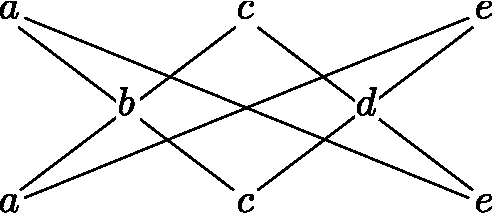
\includegraphics[width=.5\textwidth]{figures/pentagon_mu.pdf}
	\caption[Pentagon problem in multiple-unicast form]{The pentagon in multiple-unicast form. As with bipartite graphs, there are two copies of the ``external'' nodes $a$, $c$ and $e$.}
	\label{pentagon-mu}
\end{figure}

It is now clear why the new game must be imagined as two dice values, or some other example which splits the data at one node evenly between each of the two adjacent nodes. Imagine that it was not the case, and that each node transmitted a fraction $p$ to the left, and a fraction $1 - p$ to the right. To maintain the advantage described above, and for each node to receive the same amount of information, each must act consistently. Since the number of nodes is odd, one node will receive a fraction $p$ from each neighbour, meaning $p = 1 - p$ and $p = 1/2$.

\subsection{The M{\"o}bius-Band Guessing Strategy}
\label{sect:pentagon-proof}

As mentioned in Section~\ref{sect:rgg}, The guessing game played on the pentagon has a particularly elegant solution if the alphabet size is a square number, $s = t^2$. Here imagine that each player has two $t$-sided dice, numbered in the usual manner from $1$ to $t$. the two values are given as an ordered pair $(x, y) \in \{1, 2, \dots, t\}^2$. This provides an example of a network where the guessing number does indeed depend on $s$.

In the case of a pentagon, the players are assigned values $(x_i, y_i)$, for $i \in \{1, 2, 3, 4, 5\}$. Consider the guessing strategy where each player assumes that the following identities hold:
%%%%%%%%%%%%%%%%%%%%%%%%%%%
\begin{eqnarray}
  	x_1 & = & x_2 \nonumber \\
  	x_3 & = & x_4 \nonumber \\
  	x_5 & = & y_1 \nonumber \\
  	y_2 & = & y_3 \nonumber \\
  	y_4 & = & y_5. \label{eqn:mobius}
\end{eqnarray}

\newpage

This is analogous to each player assuming that one of their dice has the same value as one of their left neighbour's dice, and the other having the same value as one of their right neighbour's dice. This set of identities can be viewed geometrically as a M{\"o}bius band, by writing $x_1 = x_2, x_3 = x_4, x_5 = $ on one side of a strip of paper, $y_1, y_2 = y_3, y_4 = y_5,$ on the other side, and fix the strip together with a half-twist \cite{riis2007}, as in Figure~\ref{fig:mobius-strategy}. Note that other pairings could be used, for instance $x_i = y_{i + 1}$ for $i \in \{1, 2, 3, 4, 5\}$, where $i$ is calculated modulo $5$, provided that there is a connecting edge between the two values.

\begin{figure}[ht]
	\centering
	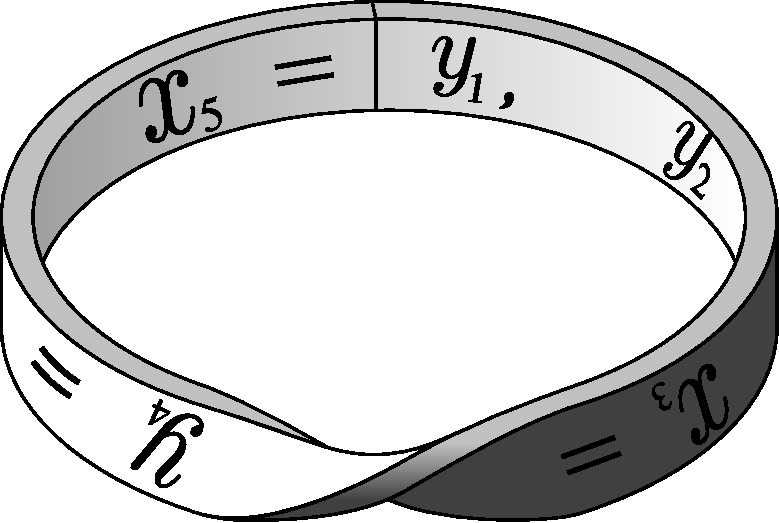
\includegraphics[width=.5\textwidth]{figures/mobius_strategy.pdf}
	\caption[The M{\"o}bius-band guessing strategy]{The M{\"o}bius-band guessing strategy is so called because it can be viewed as the set of solutions written on two sides of a strip of paper.}
	\label{fig:mobius-strategy}
\end{figure}

Using this guessing strategy on the pentagon ensures a guessing number in the half-open interval $(2, 2.5]$, with the upper bound of $2.5$ only achievable if the underlying alphabet contains a square number of letters. In other words, if the size of the alphabet is not a perfect square, then the interval is fully open. Here we have an example where the guessing number depends on $s$. This idea is expressed in Lemma~\ref{lem:mobius-lower-bound} and Lemma~\ref{lem:mobius-upper-bound}.

\begin{lemma}[\cite{riis2007}]
 \label{lem:mobius-lower-bound}
 The M{\"o}bius-band guessing strategy ensures that $k(C_5, s) \geq 5/2$ where $s = t^2, t \in \NN, t > 1$.
\end{lemma}

\begin{proof}
 Using the M{\"o}bius-band guessing strategy, the players all guess correctly when the system of equations (\ref{eqn:mobius}) hold, which happens with probability $t^{-5} = s^{-5/2}$. Since uncoordinated random guessing succeeds with probability $s^{-5}$, the guessing number is at least $5/2$.
\end{proof}

As mentioned above, this lemma requires the alphabet to contain a square number of letters. In general, a similar method can be used, and indeed will be used below, though the upper bound of $5/2$ is unachievable.

\begin{lemma}[\cite{riis2007}]
 \label{lem:mobius-upper-bound}
 The guessing number of the pentagon is at most $5/2$.
\end{lemma}

\begin{proof}
 As with the proof for the $2n$-cycle, fix any guessing protocol $\mathcal{P}$ and let $L_\mathcal{P}$ denote the set of $5$-tuples $(x_1, x_2, \dots, x_5 ) \in A^5$ for which all nodes guess correctly. Select a string at random from $L_\mathcal{P}$, and calculate the entropies of the random variables in the string, using the logarithm in base $s$, where $s = |A|$. Again using Shannon's identities:
 
\[H(x_j) \leq 1 \quad \forall j \in \{1, 2, 3, 4, 5\} \]
\[H(x_{j - 1}, x_{j}, x_{j + 1}) - H(x_{j - 1}, x_{j + 1}) = 0 \quad \forall j \in \{1, 2, 3, 4, 5\}. \]

In addition to these identities there is a joint entropy relation, rather key to Shannon's theory of information, which states that
%%%%%%%%%%%%%%%%%%%%%%%%%%%
\begin{eqnarray}
 H(A, B, C) + H(C) \leq H(A, C) + H(B, C) \label{eqn:shannon}.
\end{eqnarray}
%%%%%%%%%%%%%%%%%%%%%%%%%%%

Now letting $(A, B, C) = ( \{ x_1 \}, \{ x_3 \}, \{ x_4, x_5 \} )$, the inequality becomes
%%%%%%%%%%%%%%%%%%%%%%%%%%%
\begin{eqnarray*}
 H(x_1, x_2, x_3, x_4, x_5) + H(x_4, x_5) & = & H(x_1, x_3, x_4, x_5) + H(x_4, x_5) \\
                                          & \leq & H(x_1, x_4, x_5) + H(x_3, x_4, x_5) \\
                                          & = & H(x_1, x_4) + H(x_3, x_5) \\
                                          & \leq & H(x_1) + H(x_3) + H(x_4) + H(x_5).
\end{eqnarray*}

Thus,
%%%%%%%%%%%%%%%%%%%%%%%%%%%
\begin{eqnarray}
 H(x_1, x_2, x_3, x_4, x_5) \leq H(x_1) + H(x_3) + H(x_4) + H(x_5) - H(x_4, x_5) \label{eqn:ineq1}.
\end{eqnarray}

Next, using conditional entropy,
%%%%%%%%%%%%%%%%%%%%%%%%%%%
\begin{eqnarray*}
 H(x_1, x_2, x_3, x_4, x_5) - H(x_2, x_5) & \leq & H(x_3, x_4 | x_2, x_5) \\
                                          & = & H(x_4 | x_2, x_5) \\
                                          & \leq & H(x_4|x_5) \\
                                          & = & H(x_4, x_5) - H(x_5).
\end{eqnarray*}

This gives
%%%%%%%%%%%%%%%%%%%%%%%%%%%
\begin{eqnarray}
 H(x_1, x_2, x_3, x_4, x_5) & \leq & H(x_2, x_5) + H(x_4, x_5) - H(x_5) \nonumber \\
                            & \leq & H(x_4, x_5) + H(x_2). \label{eqn:ineq2}
\end{eqnarray}

Adding (\ref{eqn:ineq1}) and (\ref{eqn:ineq2}) we get

\[ 2H(x_1, x_2, x_3, x_4, x_5) \leq H(x_1) + H(x_2) + H(x_3) + H(x_4) + H(x_5) \leq 5. \]
\end{proof}

The same argument may be used to prove a similar theorem about odd cycles in general:

\begin{theorem}[\cite{dant2007}]
 The optimal guessing number of an undirected cycle on $2k + 1$ vertices is $k + \frac{1}{2}$.
\end{theorem}

\begin{proof}
	
 As before, setting $(A, B, C) = (\{ x_1 \}, \{ x_3, \dots, x_{2k - 1} \}, \{ x_{2k}, x_{2k + 1} \})$ in (\ref{eqn:shannon}), we have
%%%%%%%%%%%%%%%%%%%%%%%%%%%
\begin{eqnarray*}
 H(x_1, x_2, x_3, \dots, x_{2k}, x_{2k + 1}) + H(x_{2k}, x_{2k + 1}) & = & H(x_1, x_3, \dots, x_{2k}, x_{2k + 1}) + H(x_{2k}, x_{2k + 1}) \\
                           & \leq & H(x_1, x_{2k}, x_{2k + 1}) + H(x_3, \dots, x_{2k + 1}) \\
                           & \leq & H(x_1, x_{2k}) + H(x_3, x_5, \dots, x_{2k - 1}, x_{2k + 1}) \\
                           & \leq & H(x_{2k}) + \sum_{r = 0}^k H(x_{2r + 1}).
\end{eqnarray*}

This gives
%%%%%%%%%%%%%%%%%%%%%%%%%%%
\begin{eqnarray}
 H(x_1, \dots, x_{2k + 1}) \leq H(x_{2k}) - H(x_{2k}, x_{2k + 1}) + \sum_{r = 0}^k H(x_{2r + 1}) \label{eqn:dantineq1}.
\end{eqnarray}

Now setting $(A, B, C) = (\{ x_2, \dots, x_{2k - 2} \}, \{ x_{2k} \}, \{ x_{2k + 1} \})$ in (\ref{eqn:shannon}), we have
%%%%%%%%%%%%%%%%%%%%%%%%%%%
\begin{eqnarray*}
 H(x_1, \dots, x_{2k + 1}) + H(x_{2k + 1}) & = & H(x_2, \dots, x_{2k - 2}, x_{2k}, x_{2k + 1}) + H(x_{2k + 1}) \\
                           & \leq & H(x_2, \dots, x_{2k - 2}, x_{2k + 1}) + H(x_{2k}, x_{2k + 1}) \\
                           & \leq & H(x_2, x_4, \dots, x_{2k - 4}, x_{2k - 2}, x_{2k + 1}) + H(x_{2k}, x_{2k + 1}) \\
                           & \leq & H(x_{2k}, x_{2k + 1}) + H(x_{2k + 1}) + \sum_{r = 1} ^{k - 1} H(x_{2r}).
\end{eqnarray*}

Therefore,
%%%%%%%%%%%%%%%%%%%%%%%%%%%
\begin{eqnarray}
 H(x_1, \dots, x_{2k + 1}) \leq H(x_{2k}, x_{2k + 1}) + \sum_{r = 1} ^{k - 1} H(x_{2r}) \label{eqn:dantineq2}.
\end{eqnarray}

Finally, adding (\ref{eqn:dantineq1}) and (\ref{eqn:dantineq2}) we get

\[ 2H(x_1, \dots, x_{2k + 1}) \leq \sum_{r = 1} ^{2k + 1} H(x_{r}) \leq 2k + 1. \]
\end{proof}

\subsection{General Case}

As mentioned above, the guessing game has a nice solution when $s = |A|$ is a perfect square, and the guessing number of a pentagon in this case is $5/2$. In general, where the size of the alphabet is not necessarily a square, the guessing number is in the interval $(2, 2.5)$ as before. The cardinality of $L_\mathcal{P}$ is (in general) an integer.

\begin{observation}
	The guessing number of any directed graph on $n$ nodes over an alphabet of size $s$ is of the form $k = \log_s(j)$ where $j \in \NN$.
\end{observation}

From this, and using the transcendence of numbers of the form $\log_s(j)$, the following is evident:

\begin{corollary}
	Assume $s$ is not a power. Then the guessing number of a directed graph over an alphabet of size $s$ is either an integer or an irrational number. If, on the other hand, $s = t^k$ where $t$ is not a power, each directed graph has either a guessing number of the form $r/k$ where $r \in \NN$, or is irrational.
\end{corollary}

\subsection{Example}

To illustrate the above observation, the simplest example is used here: the case of the pentagon where the underlying alphabet has size $2$; $A = \{0, 1\}$. The guessing number is of the form $\log_2(j)$. Since the guessing number is at least $2$ and at most $5/2$, there are only two possible values, where $j = 4$ and $j = 5$, giving guessing numbers of $2$ and $\log_2(5) \approx 2.32$. There is actually a strategy that ensures a guessing number of $\log_2(5)$: All players guess with the assumption that there are never two consecutive $1$s or three consecutive $0$s. There are exactly five $5$-tuples that satisfy these assumptions, namely $(0, 0, 1, 0, 1)$, $(0, 1, 0, 0, 1)$, $(0, 1, 0, 1, 0)$, $(1, 0, 0, 1, 0)$ and $(1, 0, 1, 0, 0)$. This strategy also uniquely determines the values available to the players from their neighbours. The guessing strategy succeeds with probability $5/32$, or $5$ times more successful than random guessing. Therefore, the guessing number of the pentagon for $s = 2$ is $\log_2(5)$.

\subsection{Three-Layers Argument}

The three-layers argument is useful as a pictorial description of the message pairing process used in the M{\"o}bius-band guessing strategy. In the case of even cycles, it is not possible to improve on the node-pairing method. To show that it is not possible to improve on a guessing number of $n$ for a $2n$-cycle, consider a pattern where every evenly numbered node is fixed, so the odd-numbered nodes can be uniquely determined.

As in Section~\ref{sect:pentagon-proof} above, each node in a pentagon is assigned two values $(x_i, y_i)$, for $i \in \{1, 2, 3, 4, 5\}$, and $x_i = y_{i + 1}$ for $i \in \{1, 2, 3, 4, 5\}$, where $i$ is calculated modulo $5$. Now, split all nodes $x_i$ as with a bipartite graph, leaving nodes $y_i$ as ``internal'' nodes. The initial and resulting graphs are shown in Figure~\ref{fig:3layers}.

\begin{figure}[ht]
     \centering
     \subfigure[]{
          \label{fig:3layers-before}
          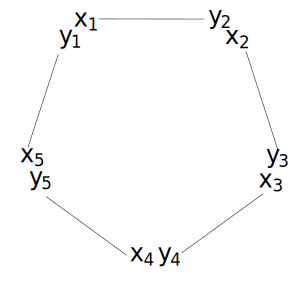
\includegraphics[width=.45\textwidth]{figures/3layers-before.pdf}}
     \hspace{.3in}
     \subfigure[]{
          \label{fig:3layers-after}
          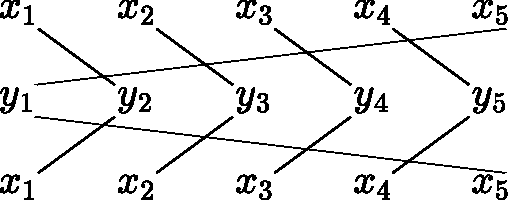
\includegraphics[width=.45\textwidth]{figures/3layers-after.pdf}}
     \caption[Three-layers argument before and after conversion]{Each node of the pentagon \subref{fig:3layers-before} is assigned two values. Nodes $x_i$ are then split as in a bipartite graph to give the three-layered graph \subref{fig:3layers-after}. As with bipartite graphs, edges are directed downwards.}
     \label{fig:3layers}
\end{figure}

This argument seems to show quite well what happens when considering that each node has two messages to resolve.

\section{Summary}

This chapter contains the main theorems resulting from the new guessing game. The proofs of these theorems are also included, and centre mainly around the use of Shannon's inequalities to determine the guessing numbers of particular graphs, specifically undirected cycles. Two key observations are made about the properties of guessing numbers under certain conditions in the new game; finally, the observations are illustrated with a simple example.